\documentclass{ctexart}
% 数学公式
\usepackage{amsmath, amssymb, mathtools}
%处理图片
\usepackage{graphicx}
\usepackage{float}
\usepackage{subfigure}
% 页面设置
\pagestyle{plain}
\usepackage[a4paper, top=1in, bottom=1in, left=1.5in, right=1.5in]{geometry}
\usepackage[fontsize=12]{fontsize}
% 文档内容
\begin{document}

\title{深入理解控制理论}
\author{ecstayalive}
\maketitle

\section*{控制理论基本概念 Why?}
在此之前,我们需要理解这句话:关于现实中的自然现象,我们可以使用微分方程来近似描述。
要深刻的解释这一点很不容易,但是我们应该知道,我们的目的是解释自然现象符合的方程,其中
可以使用微积分这个工具来近似的描述自然的变化,因此微分方程似乎是一个合理的选择。

\subsection*{微分方程}
好了现在我们已经知道了任何一个物理系统其所符合的规律可以使用一个微分方程来描述。为了简化
问题,我们假设该物理系统有一个输入$x$与一个输出$y$,并且我们通过一些分析发现他们符合如下
的微分方程式:

\begin{equation}
    a_n \frac{d^n y(t)}{d t^n} +
    \cdots + a_1 \frac{d y(t)}{dt} + a_0 y(t)
    = b_m \frac{d^m x(t)}{d t^m} +
    \cdots + b_0 x(t)
    \label{eq:1}
\end{equation}

这个公式很抽象,现在让我们举一个简单的例子:

%H为当前位置,!htb为忽略美学标准,htbp为浮动图形
\begin{figure}[H]
    %图片居中
    \centering
    %插入图片,[]中设置图片大小,{}中是图片文件名
    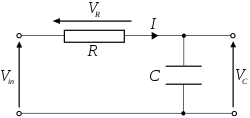
\includegraphics[width=0.45\textwidth]{./pics/deeply_understand_control_theory/1.png}
    %最终文档中希望显示的图片标题
    \caption{简单RC电路}
    %用于文内引用的标签
    \label{Fig.1}
\end{figure}

如图\ref{Fig.1}所示,这是一个简单的RC电路,明显其输入为$V_{in}$其输出为$V_c$,
同时我们知道对于电容$C$符合如下的微分方程:

\begin{equation}
    I = C \frac{d V_c}{d t}
    \label{eq:2}
\end{equation}

所以对于该系统如果以$V_{in}$为输入,以$V_c$为输出,则我们可以通过如下的微分方程描述
该系统:

\begin{equation}
    RC \frac{d V_c}{d t} + V_c = V_{in}
    \label{eq:3}
\end{equation}

而这个微分方程就类似于公式\eqref{eq:1}的形式。

\textbf{所以请记住,微分方程是描述系统的最基本的形式,如果我们计算能力足够强大,
    掌握这个微分方程就足以分析、描述与预测该系统了}

\subsubsection*{零状态响应与零输入响应}
这是经常混淆的两个概念,现在就让我们讨论一下。

首先什么是零状态响应呢?用比较学术的文字描述就是指一个系统,其内部动态元件初始储能为零,
完全由外部输入激励引起的响应。什么意思呢?举个例子就是,如果只给定了一个微分方程,我们
可以解出来无穷多个解——通解。可是现实并不是这样,就比如对于图\ref{Fig.1}描述的系统,
我们给定一个$V_{in}$,只会观察出来一种输出。也就是说对于我们真正有用的是符合一定初始
条件的特解。只不过是,零状态响应,规定了初始状态为0。

就比如图\ref{Fig.1}描述的系统的零状态响应,就是我刚开始建成电路,内部没有任何能量。
在我通上电后,就得到了一个输出。如何求解这个输出呢?只需要求解满足初始状态为0的特解就
可以。即解决如下的方程:
\begin{equation}
    \begin{array}{rl}
        \text{solve:}      & RC \frac{d V_c}{d t} + V_c = V_{in} \\
        \text{subject to:} & V_c = 0, V_{in} \neq 0
    \end{array}
    \label{eq:4}
\end{equation}

求出的特解便是系统的零状态响应。

那何为零输入响应呢?其实就是对于一个系统,内部依然存有激励,而无外部激励得到的输出曲线。
例如,对于图\ref{Fig.1}描述的简单RC系统,其实就是内部状态不为0,但是其输入为0,
即解决如下的方程求出特解即为系统的零输入响应。

\begin{equation}
    \begin{array}{rl}
        \text{solve:}      & RC \frac{d V_c}{d t} + V_c = 0 \\
        \text{subject to:} & V_c \neq 0
    \end{array}
    \label{eq:5}
\end{equation}

你会发现,微分方程已经包含了零状态响应与零输入响应,只不过我们要确定初值条件,来
得到符合现实情况的输入曲线。当然对于一个线性系统而言,由于其符合叠加性与齐次性,
因此我们可以把一个既带有内部激励又带有外部输入的系统分解为两个子系统,第一个便是
零状态响应系统,即没有内部激励,但有外部输入。第二个便是零输入响应,即有内部激励,
但是没有外部输入。这样整体系统的响应输出便是这两个子系统的响应输出之和。但是,
千万记住,这一切都是可以从\textbf{微分方程}这里得到的。


\subsection*{Laplace变换}
那么为什么要使用Laplace变换呢?一部分原因是我们计算太弱了,我们可以分析得到系统
说符合的微分方程,但是要计算出来这个特解却很难。也就是说在时域中计算现实中的输出太难了,
因为我们使用Laplace变换帮助我们稍微简化这个过程。
所以千万记住,Laplace时用来计算特解的,也就是说Laplace变换本身就是和系统变量的初始值
有关系的。这一点从Laplace变换上就可以体现出来,例如:

\begin{equation}
    \mathbf{L}[\frac{d f(t)}{dt}] = s F(s) - f(0_{\pm})
    \label{eq:6}
\end{equation}

其中,$f(0_{\pm})$就是一个系统变量的初值。从这里看出,Laplace是帮助我们解决微分方程
特解的。但是,通常我们分析的系统往往没有内部激励,因此我们引入了传递函数这个概念,即
\textbf{在零状态响应的条件下}, 输出信号的Laplace变换与输出信号的Laplace变换的比值。
这时,$f(0_{\pm})=0$。也因此,求解传递函数时,系统内部本身的激励信号被值为0了。
也因此,假设系统内部有激励信号,我们必须通过传递函数得到系统的基本微分方程,在设置初值过后,
再次利用Laplace变换得到输出响应。

举一个例子,就比如图\ref{Fig.1}所示的系统,很简单,我们已知其传递函数是:

\begin{equation}
    \frac{V_c(s)}{V_{in}(s)} = \frac{1}{1 + RCs}
    \label{eq:7}
\end{equation}

然后假设我们需要求$V_{c}$初始值为1的情况下的系统输出响应,很遗憾我们没有办法,我们
需要先通过这个公式\eqref{eq:7}写出其微分方程,然后再次使用Laplace得到$V_{c}(0)=1$
情况下的Laplace变换:

\begin{gather}
    RC \frac{d V_c}{d t} + V_c = V_{in} \notag\\
    RCs V_c(s) - 1 + V_c(s) = V_{in}(s)     \\
    V_c(s) = \frac{V_{in}(s) + 1}{RCs + 1} \notag
    \label{eq:8}
\end{gather}

从这里看出,传递函数虽然忽略了系统内部变量的初始值,不能求出在非零初始值情况下系统的输出,
但是却可以得到系统的基本微分方程,反映了系统自身的特性。

同时啊,值的注意的是,由于单位脉冲函数的Laplace变换是1,即$\mathbf{L}[\delta(t)]=1$,
这也就意味着,在零状态条件下,当输入是单位脉冲函数时,
有$V_{out}(s) = G(s) \cdot 1 = G(s)$,即响应输出的Laplace变换就是系统的传递函数。

\section*{系统输入与输出}

\subsection*{系统输入函数}

在前一节我们讨论了控制理论的基本概念,并且理解了为什么这样做,以及方法的限制性与目的。
这一小节我们讨论一个常常被人忘记的东西,输入函数。由于我们引入了传递函数概念,其可以
反映系统本身的特性,并且通常,在连续域控制中,这种特性与系统本身输入往往没有关系。
所以我们不会关注输入是怎么样的。但是问题在于如果我们想要知道一个系统本身的输出,就必然
给定输入。

自然界中的输入函数复杂多样,难以寻找规律,因此我们在这里仅仅讨论一下一些基本的输入函数,
并如何通过这些基本的输入函数构建复杂的输入函数。又因为我们熟知的脉冲函数,单位阶跃函数,
单位斜坡函数,单位抛物线函数,三角函数的图像十分简单,因此为节约时间我们不在详细讲述。
那么接下来,让我们关注如何通过这些函数获得一些复杂的输入函数。下面为基本输入函数图像的
示例。

%H为当前位置,!htb为忽略美学标准,htbp为浮动图形
\begin{figure}[H]
    \centering
    \begin{minipage}{\textwidth}
        \centering
        % subfigure[图片描述]{图片}
        \subfigure[单位阶跃函数]{
            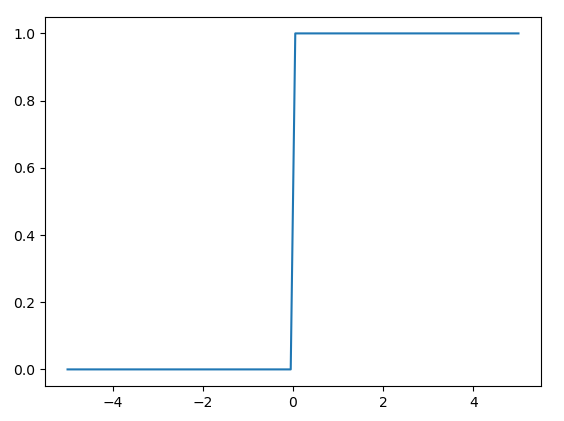
\includegraphics[width=0.45\textwidth]{./pics/deeply_understand_control_theory/step.png}
        }
        % repeat subfigure
        \centering
        % subfigure[图片描述]{图片}
        \subfigure[单位斜坡函数]{
            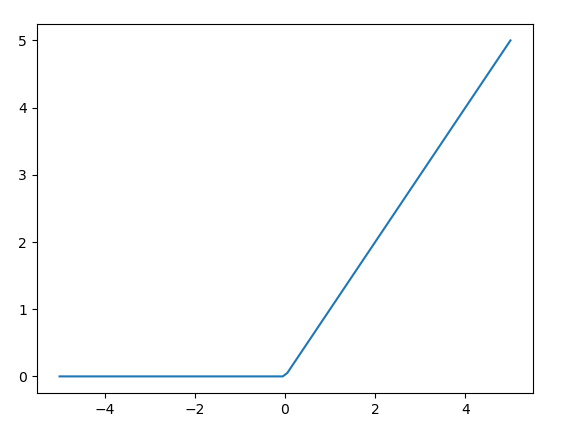
\includegraphics[width=0.45\textwidth]{./pics/deeply_understand_control_theory/velocity.png}
        }
        \centering
        % subfigure[图片描述]{图片}
        \subfigure[单位加速度函数]{
            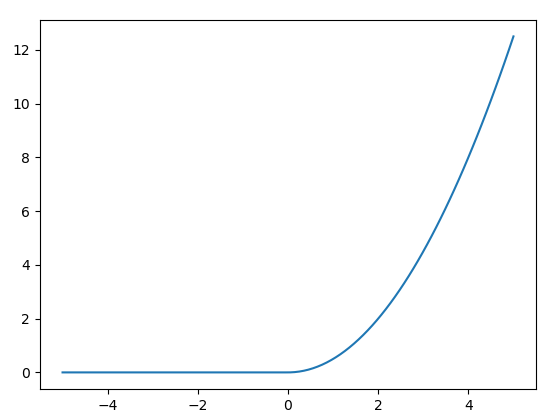
\includegraphics[width=0.45\textwidth]{./pics/deeply_understand_control_theory/acceleration.png}
        }
        \centering
        % subfigure[图片描述]{图片}
        \subfigure[sin函数]{
            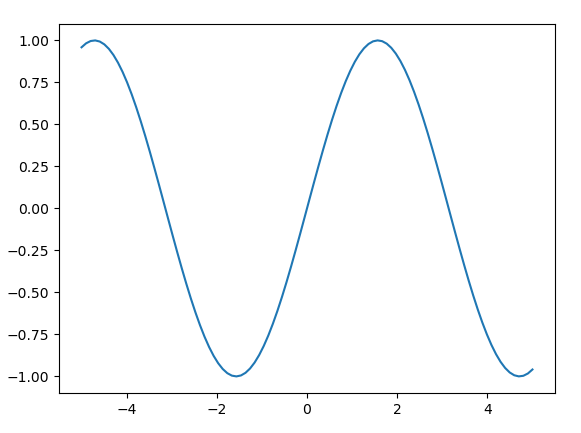
\includegraphics[width=0.45\textwidth]{./pics/deeply_understand_control_theory/sin.png}
        }

    \end{minipage}
    % repeat minipage

    \caption{基本输入函数}
    \label{Fig:2}
\end{figure}

在此介绍一种得到一些复杂函数的基本方法,平移方法。举个简单的例子,例如下面的矩形波函数
我们该如何构建呢?简单我们已知一个与其很像的函数——单位阶跃函数$u(t)$,但是$u(t)$在$t>1$
后依然是存在的,为了消除这一部分影响,我们先把$u(t)$向左平移一个单位得到一个函数
$u(t - 1)$,然后这两个函数相减便可以得到一个矩形波函数,如下面三幅图所示:
%H为当前位置,!htb为忽略美学标准,htbp为浮动图形
\begin{figure}[H]
    \centering
    \begin{minipage}{\textwidth}
        \centering
        % subfigure[图片描述]{图片}
        \subfigure[阶跃函数]{
            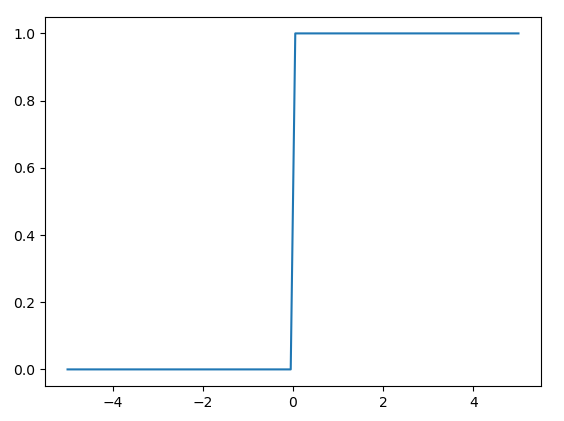
\includegraphics[width=0.45\textwidth]{./pics/deeply_understand_control_theory/step.png}
        }
        % repeat subfigure
        \centering
        % subfigure[图片描述]{图片}
        \subfigure[阶跃函数向后平移一个单位]{
            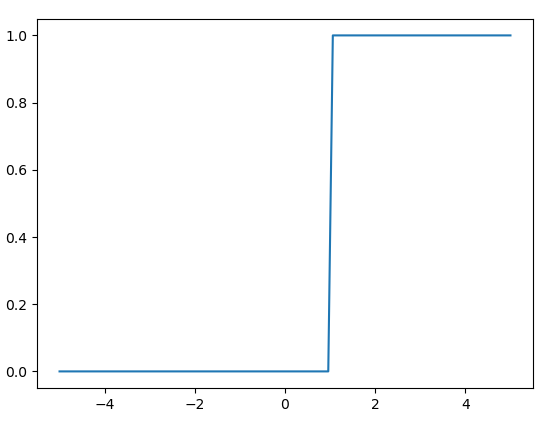
\includegraphics[width=0.45\textwidth]{./pics/deeply_understand_control_theory/step_move_1.png}
        }
        \centering
        % subfigure[图片描述]{图片}
        \subfigure[两者相减得到矩形波]{
            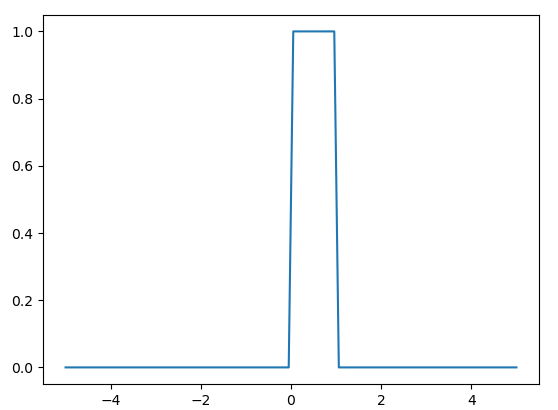
\includegraphics[width=0.5\textwidth]{./pics/deeply_understand_control_theory/rectangle.png}
        }

    \end{minipage}
    % repeat minipage
    \caption{一个函数构建的例子}
    \label{Fig:3}
\end{figure}

再比如,我们已经知道了如下的图形,如何使用基本函数构建呢?
%H为当前位置,!htb为忽略美学标准,htbp为浮动图形
\begin{figure}[H]
    %图片居中
    \centering
    %插入图片,[]中设置图片大小,{}中是图片文件名
    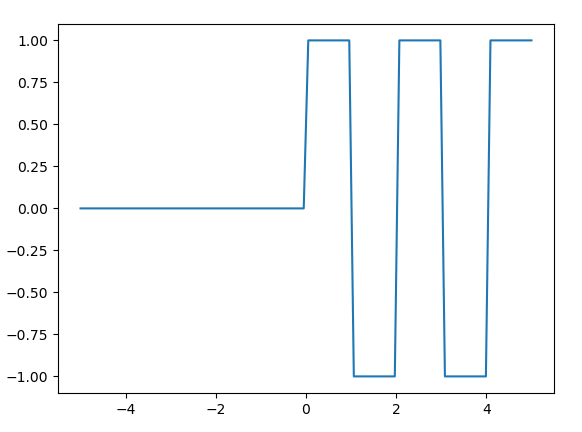
\includegraphics[width=0.55\textwidth]{./pics/deeply_understand_control_theory/square_wave.png}
    %最终文档中希望显示的图片标题
    \caption{方波}
    %用于文内引用的标签
    \label{Fig.4}
\end{figure}

我们先来分析一下,明显其是由单位阶跃函数构建而来,只不过是在$t=1$是其减去了两倍的单位阶跃函数,
用数学公式描述即:

\begin{equation}
    y(t) = u(t) - 2u(t-1)
\end{equation}

此时图像变为了:

%H为当前位置,!htb为忽略美学标准,htbp为浮动图形
\begin{figure}[H]
    %图片居中
    \centering
    %插入图片,[]中设置图片大小,{}中是图片文件名
    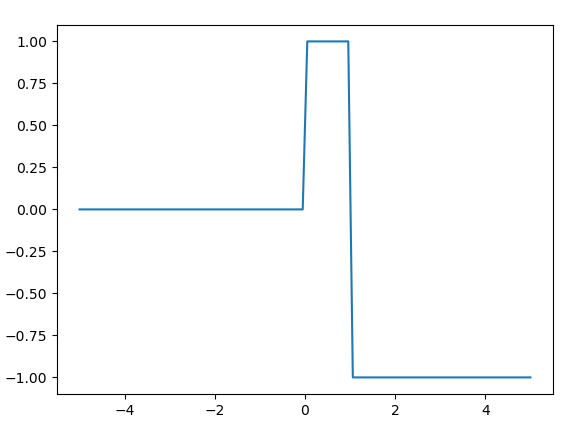
\includegraphics[width=0.55\textwidth]{./pics/deeply_understand_control_theory/step_transform1.png}
    %最终文档中希望显示的图片标题
    \caption{变换1}
    %用于文内引用的标签
    \label{Fig.5}
\end{figure}

接着在$t=2$时,又加上了一个两倍的像右平移两个单位的单位阶跃函数,即:

\begin{equation}
    y(t) = u(t) - 2u(t-1) + 2u(t-2)
\end{equation}

此时图像变为了:

%H为当前位置,!htb为忽略美学标准,htbp为浮动图形
\begin{figure}[H]
    %图片居中
    \centering
    %插入图片,[]中设置图片大小,{}中是图片文件名
    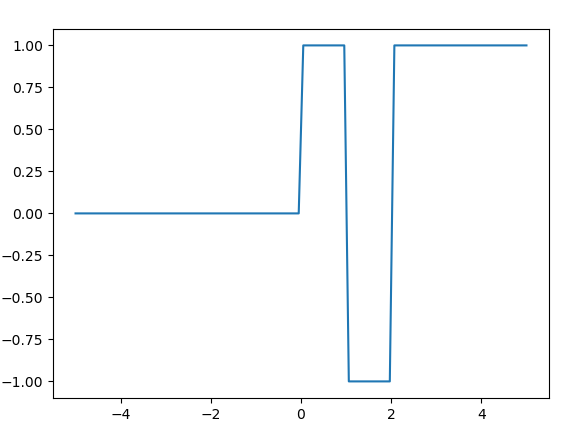
\includegraphics[width=0.55\textwidth]{./pics/deeply_understand_control_theory/step_transform2.png}
    %最终文档中希望显示的图片标题
    \caption{变换2}
    %用于文内引用的标签
    \label{Fig.6}
\end{figure}

重复这一步骤,我们便可以得到这个方波。

同时我们使用这种平移方法可以得到一些由基本函数构建得到的复杂函数,这些复杂函数往往在工程中有很大的应用。

\subsection*{输出}
在上一小结,我们已经知道了构建复杂的输入函数,但是如何求输出呢?

这个问题十分简单,因为我们可以使用上一节讲的Laplace变换来求解输出。当然我们需要注意,如果输入是简单
函数,题目中所示的系统可能不是零状态条件。但是往往如果输入是一个复杂的函数,题目往往不会这么复杂。

为了形象的展示,我们举一个例子,就比如你们问的这道题目。

%H为当前位置,!htb为忽略美学标准,htbp为浮动图形
\begin{figure}[H]
    %图片居中
    \centering
    %插入图片,[]中设置图片大小,{}中是图片文件名
    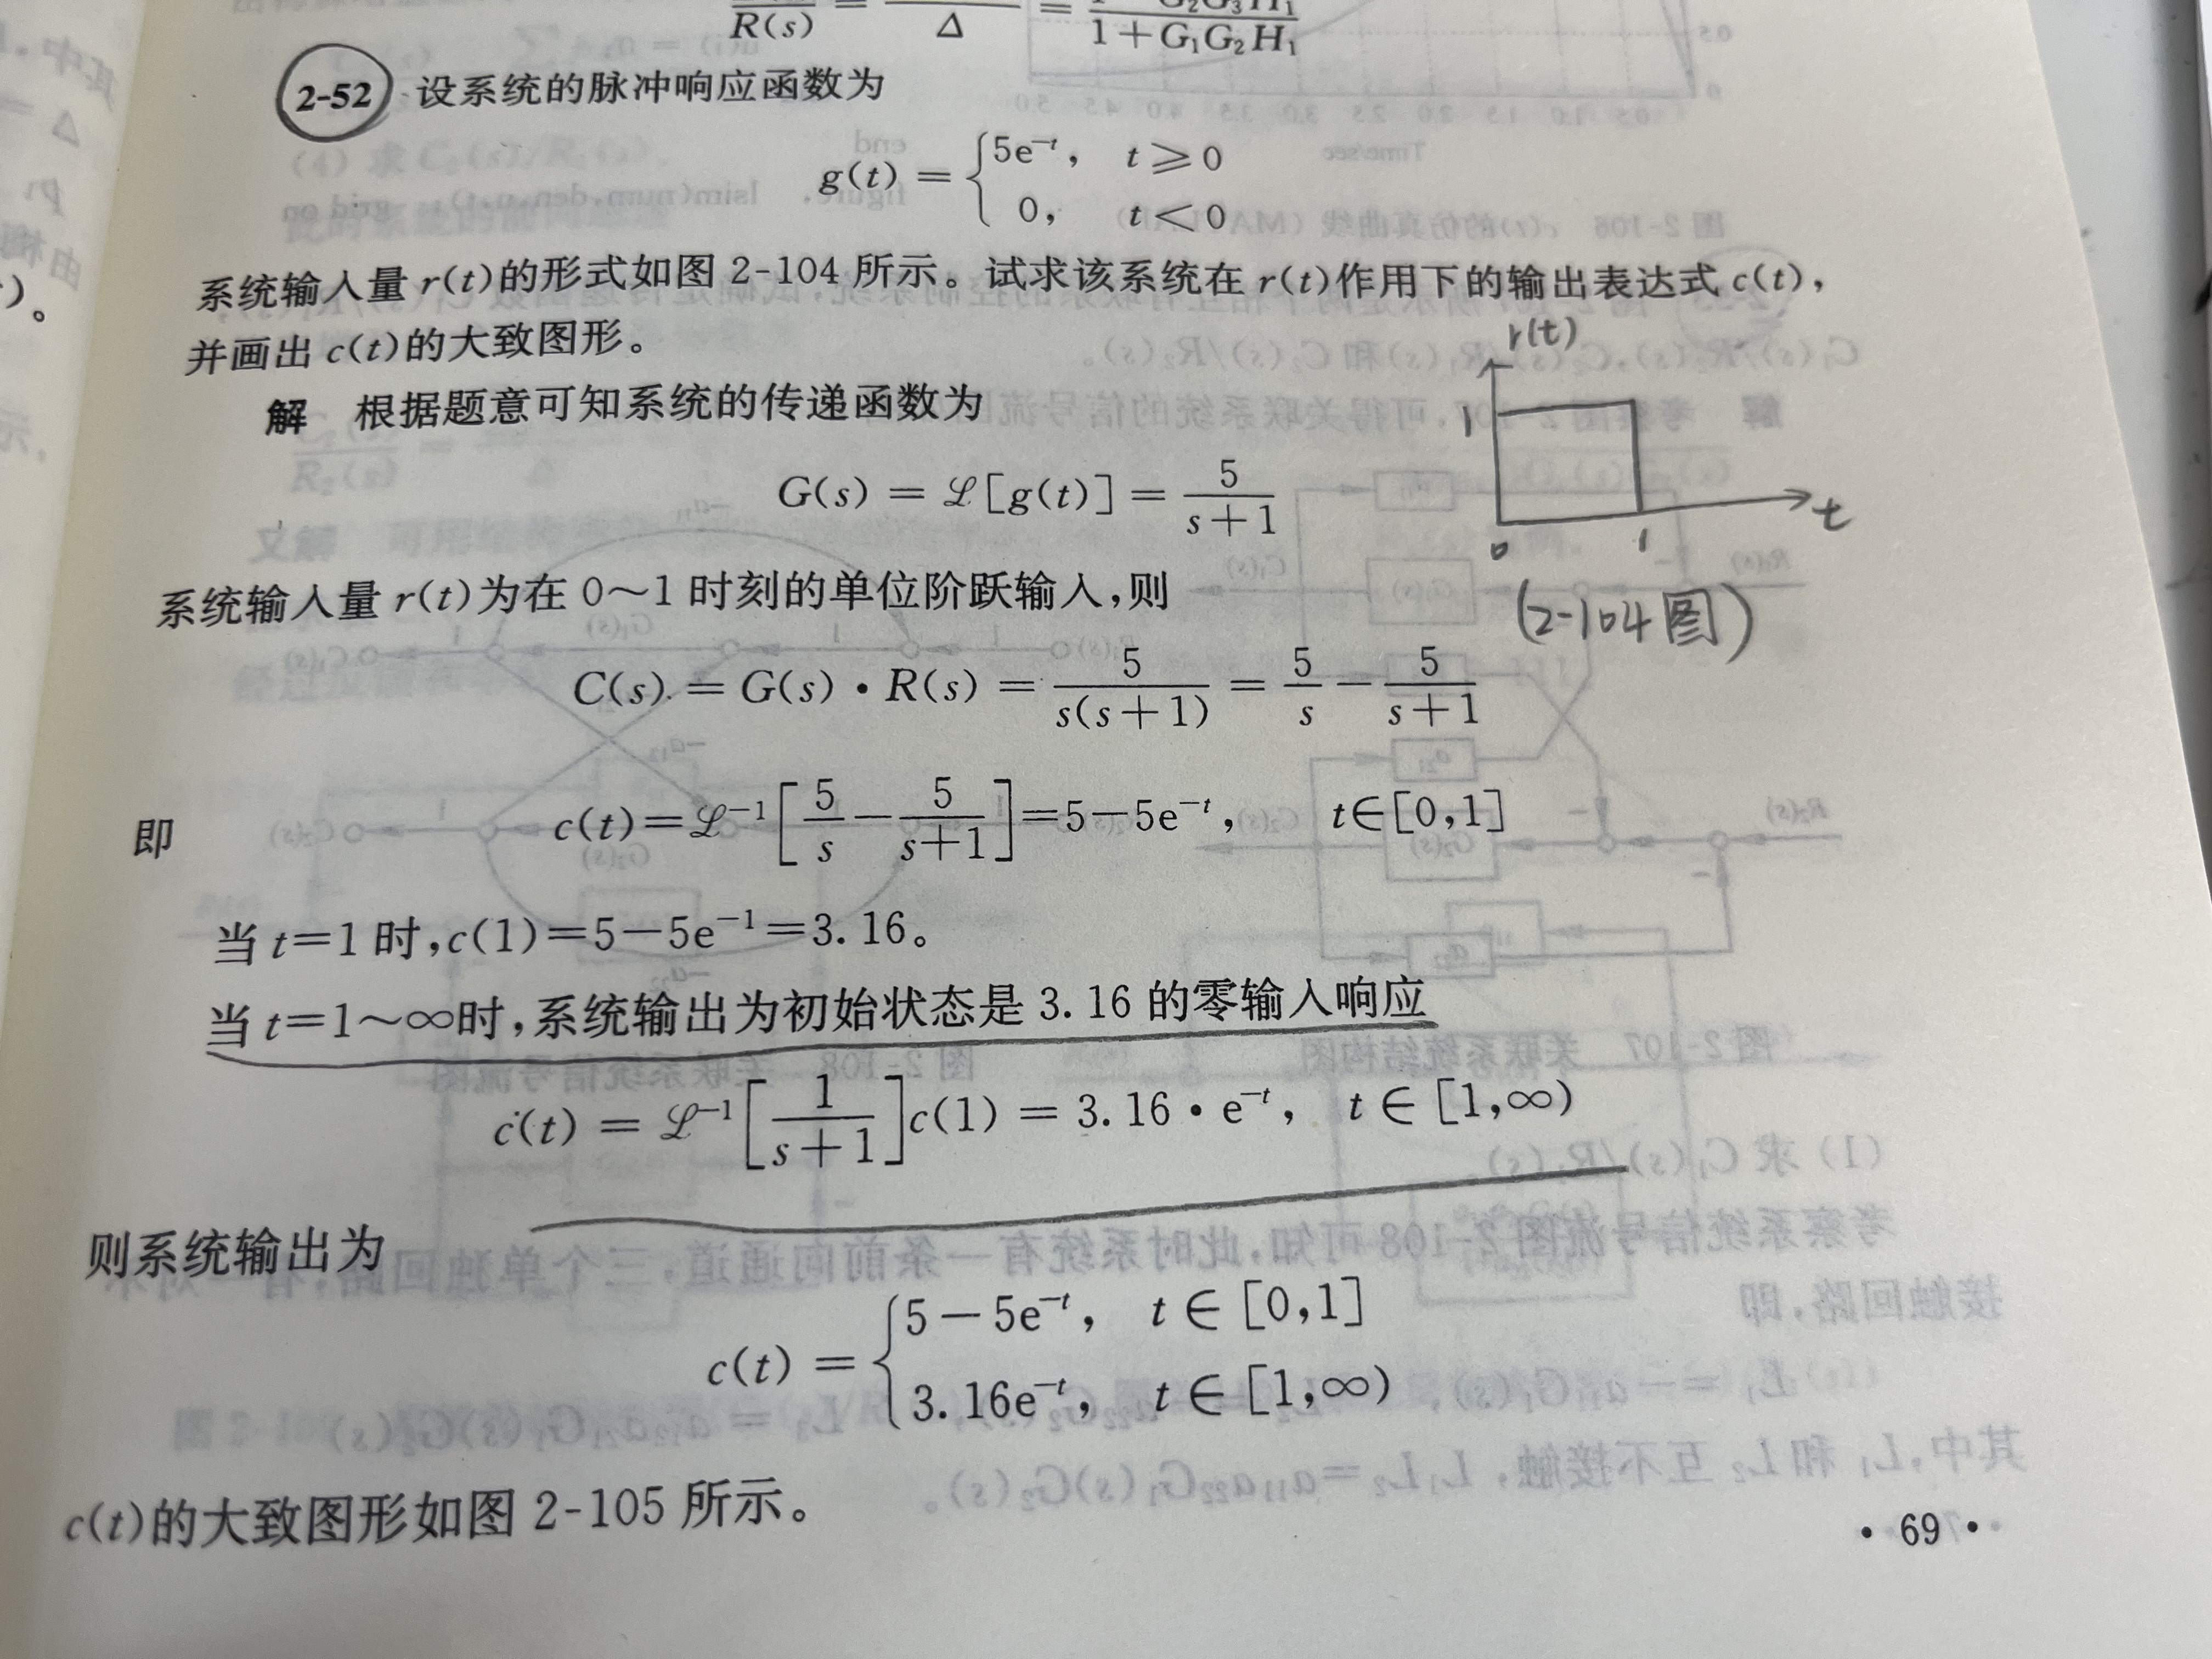
\includegraphics[width=0.99\textwidth]{./pics/deeply_understand_control_theory/example1.jpg}
    %最终文档中希望显示的图片标题
    \caption{一道例题}
    %用于文内引用的标签
    \label{Fig.7}
\end{figure}

我们已经知道了系统脉冲响应函数$g(t)$,那么根据之前所讲的我们便可以知道系统传递函数
$G(s) = \frac{5}{s + 1}$。同时我们根据平移法构建出来了输入函数$x(t) = u(t) - u(t-1)$。
其中$u(t)$为单位阶跃函数。
由于我们可以使用Laplace变换进行简化特解的计算,所以我们先进行Laplace变换得到
$X(s) = \frac{1}{s} - \frac{1}{s} e^{-s}$。进而我们得到了输出的Laplace变换:

\begin{equation}
    \begin{aligned}
        Y(s) & = G(s) X(s)                                         \\
             & = \frac{5}{s + 1}(\frac{1}{s} - \frac{1}{s} e^{-s}) \\
             & =\frac{5}{s(s + 1)}(1 - e^{-s})
    \end{aligned}
    \label{eq:11}
\end{equation}

虽然我们第一眼看过去可能觉得这个$Y(s)$无法进行Laplace反变换,但是事实确是非常简单。
我们只需要通过一般的方法拆开就会发现这个的反变换如此直观,如下:
\begin{gather}
    Y(s) = \frac{5}{s(s + 1)}(1 - e^{-s}) \\
    Y(s) = (\frac{5}{s} - \frac{5}{s+1}) (1 - e^{-s}) \\
    Y(s) = (\frac{5}{s} - \frac{5}{s+1}) - (\frac{5}{s} - \frac{5}{s+1}) e^{-s}
\end{gather}

然后我们就会发现,最后的式子可以分解为两项,这两项的Laplace反变换互不影响。只不过后一项的Laplace
反变换需要加上一个延迟环节。
\begin{equation}
    \mathbf{L^{-1}}[\frac{5}{s} - \frac{5}{s+1}] = 5u(t) - 5e^{-t}u(t)
\end{equation}

也因此,后一项的Laplace反变换为:
\begin{equation}
    \mathbf{L^{-1}}[(\frac{5}{s} - \frac{5}{s+1}) e^{-s}] = 5u(t-1) - 5e^{-(t-1)}u(t-1)
\end{equation}

所以我们可以得到$y(t)$的表达式:
\begin{equation}
    y(t) = [5u(t) - 5e^{-t}u(t)] - [5u(t-1) - 5e^{-(t-1)}u(t-1)]
\end{equation}

其实这时候,输出已经得到了,但是并不直观,虽然我们完全可以这样写,并且这是对的。
现在我们让其更加直观一点,我们先讨论$0<t<1$时,此时:
\begin{equation}
    \begin{aligned}
        y(t) & = [5u(t) - 5e^{-t}u(t)] - [5u(t-1) - 5e^{-(t-1)}u(t-1)] \\
             & = [5 - 5e^{-t}] - 0                                     \\
             & = 5 - 5 e^{-t}
    \end{aligned}
\end{equation}

当$t\geq1$时,我们可以得到系统输出:

\begin{equation}
    \begin{aligned}
        y(t) & = [5u(t) - 5e^{-t}u(t)] - [5u(t-1) - 5e^{-(t-1)}u(t-1)] \\
             & = [5 - 5e^{-t}] - [5 - 5e^{-(t-1)}]                     \\
             & = 8.59 e^{-t}
    \end{aligned}
\end{equation}

从而我们得到了一个更加直观的写法,虽然我们完全可以不这样写:
\begin{equation}
    y(t) = \begin{cases}
        5 - 5 e^{-t} & 0<t<1   \\
        8.59 e^{-t}  & t\geq 1
    \end{cases}
\end{equation}

事实上,通过这种方法我们能够轻易的写出来一下复杂的输入函数,并求出其系统响应输出。

\end{document}
